\chapter{Summary}\label{ch:summary}


\section{Results}\label{sec:results}

Presented model was trained and tested using various parameters.
The changes were affected by the input data as well as the network parameters.
The final dataset properties used to train presented model are describe in \mbox{Tab.~\ref{tab:dataset}}.
The input picture size was forced by used transfer learning model.
This limitation had an effect on resizing original pictures of sequences to the required one by the used neural network.

\begin{table}[!hbt]
    \centering
    \begin{minipage}{.49\textwidth}
        \centering
        \captionsetup{width=\linewidth}
        \captionof{table}{Dataset properties} \label{tab:dataset}
        \begin{tabular}{p{0.6\textwidth}p{0.29\textwidth}}
            \hline
            Users                    & 46                 \\ \hline
            Human users              & 45                 \\ \hline
            Bot users                & 1                  \\ \hline
            Sequences                & 639                \\ \hline
            Minimal sequence length  & 50                 \\ \hline
            Model input picture size & 299 x 299 {[}px{]} \\ \hline
        \end{tabular}
    \end{minipage}
    \hfill
    \begin{minipage}{.5\textwidth}
        \centering
        \captionsetup{width=\linewidth}
        \captionof{table}{Confusion matrix values} \label{tab:confusion-matrix}
        \begin{tabular}{p{0.50\textwidth}p{0.12\textwidth}}
            \hline
            False negatives       & 19    \\ \hline
            False positives       & 0     \\ \hline
            True negatives        & 327   \\ \hline
            True positives        & 0     \\ \hline
            False rejection rate  & 100\% \\ \hline
            False acceptance rate & 0\%   \\ \hline
        \end{tabular}
    \end{minipage}
\end{table}

The total amount of sequences depended on the minimal sequence length, because sequences that were shorter than \num{50} were simply rejected.
The minimal sequence length was fixed based on several attempts.
Shorter sequences resulted in apparently lower accuracy, when longer did not improve performance at all.
The length of \num{50} seemed to be the golden mean between accuracy and amount of sequences.

The charts presented below \mbox{(Fig.~\ref{fig:accuracy}, Fig.~\ref{fig:loss})} show that model accuracy reaches the level of \num{94}\% with \num{69.5}\% value of loss function.
It can be seen that model accuracy during the testing part is in most epochs higher than the one in the training.
It is caused by an imbalanced dataset which was the input for the presented model.
The amount of user data for testing was greater than the bot one.
It is direct effect of having more user data in the whole dataset.
The impact is also seen on the lost function chart \mbox{(Fig.~\ref{fig:loss})} where values are lower in the testing part.

\begin{figure}[!hbt]
    \centering
    \begin{minipage}{.5\textwidth}
        \centering
        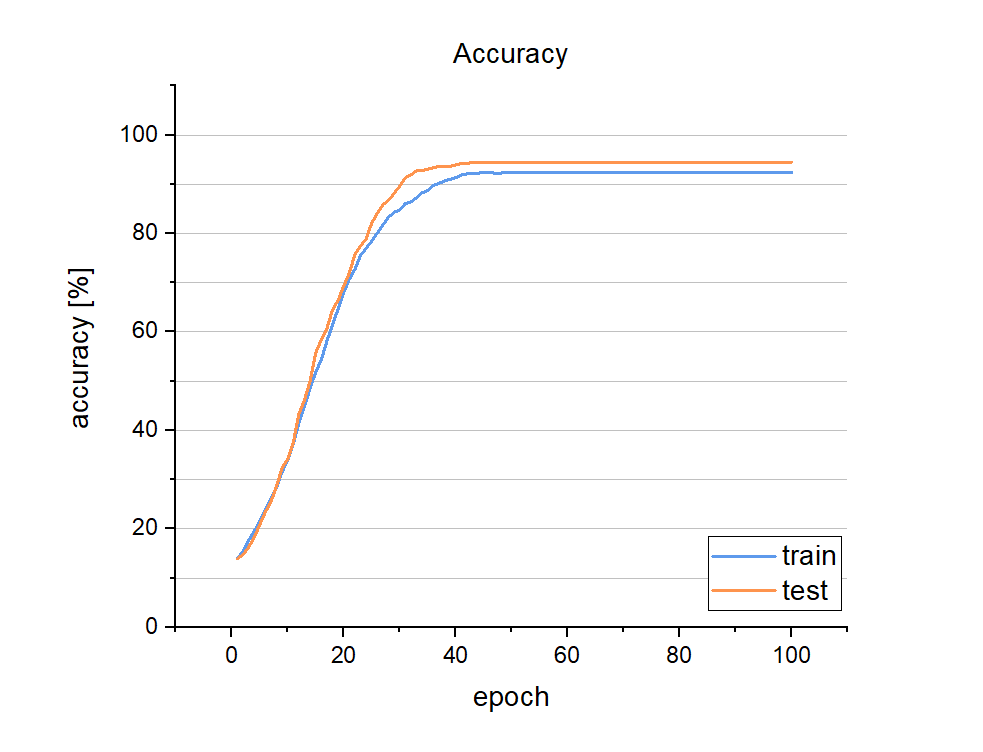
\includegraphics[width=\linewidth]{resources/accuracy.png}
        \captionsetup{width=\linewidth}
        \captionof{figure}{Accuracy of presented model}
        \label{fig:accuracy}
    \end{minipage}%
    \begin{minipage}{.5\textwidth}
        \centering
        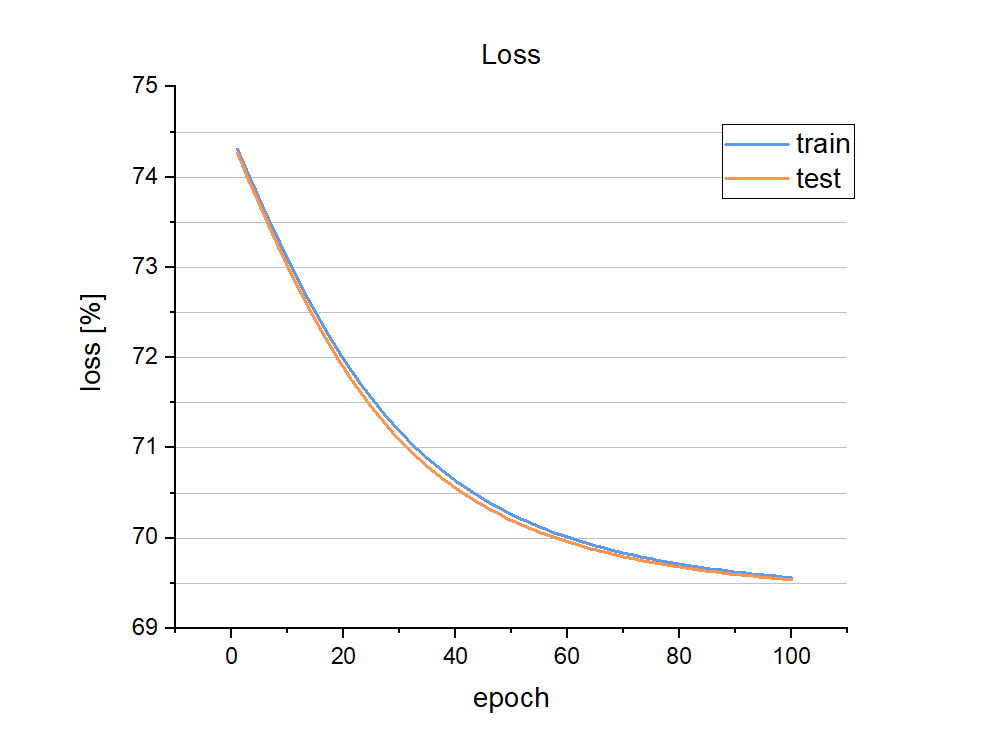
\includegraphics[width=\linewidth]{resources/loss.png}
        \captionsetup{width=\linewidth}
        \captionof{figure}{Value of loss function used in model}
        \label{fig:loss}
    \end{minipage}
\end{figure}

Moreover, due to that inappropriate data, model had some problems with prediction.
At the beginning of the learning procedure, user and bot data were treated with equal importance.
With the successive epochs, user data outshone bot dataset.
It can be seen \mbox{(Tab.~\ref{tab:confusion-matrix})} that after the learning process, there were no true positives, which suggests that the model learned only one type of data.
The model always predicted that the input data was the user's one.
It is the result of a large amount of user data in comparison to bot sequences.
It is not the result of having only one bot user and many human users, because each user's sequence was joined into a global one.

Comparing the achieved results to the ones from the original paper~\cite{Main}, the presented solution behaves unilaterally.
In many cases from cited work, authors achieved very low values of FRR\footnote{False Rejection Rate} and FAR\footnote{False Acceptance Rate}\@.
In this work, using CNN's\footnote{Convolutional Neural Network} as a core of a solution, it was achieved totally different results.
The authors consider the imbalanced dataset as the main foundation of that unexpected behavior.
Despite the numerous efforts of the authors, the results are unsatisfactory.
The obtained accuracy chart (Fig.~\ref{fig:accuracy}) is somehow expected due to the dominance of one kind of data in the binary selection problem.
However loss function (Fig.~\ref{fig:loss}) as well as confusion matrix (Tab.~\ref{tab:confusion-matrix}) have undesirable values.
